\begin{figure}[t]
	\begin{subfigure}{.49\textwidth}
	  \centering
	  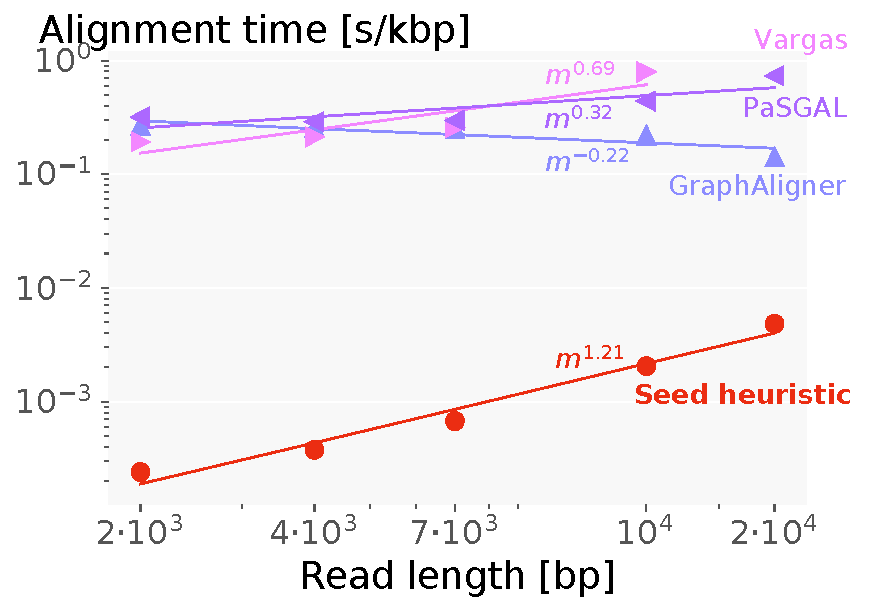
\includegraphics[width=\linewidth]{figures/hifi_spkb_vs_readlen-mxspkb.pdf}
	\end{subfigure}%
	\begin{subfigure}{.45\textwidth}
	  \centering
	  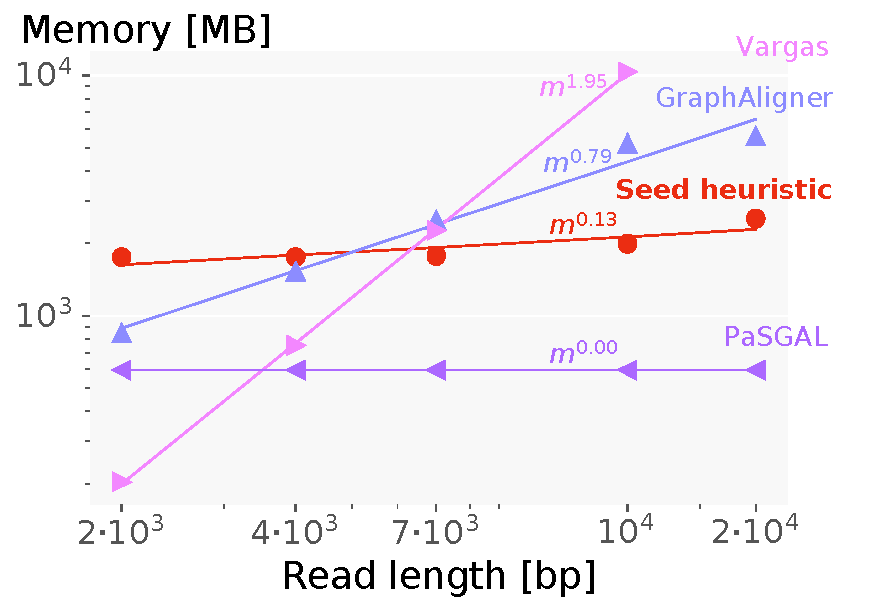
\includegraphics[width=\linewidth]{figures/hifi_memory_vs_readlen-mxmax_rss.pdf}
	\end{subfigure}~\hspace{1em} \caption{Performance degradation with HiFi read
	 length. Log-log plots of total alignment time (left) and memory usage (right)
	 show the scaling difference between aligners.}
	\label{SEEDfig:hifi_scaling_with_readlen}
  \end{figure}

\subsection{Q3: Scaling with read length}

\cref{SEEDfig:hifi_scaling_with_readlen} shows the runtime and memory scaling with
increasing length of aligned HiFi reads on MHC reference. Here we used reads
with a total length of 100Mbp for the \seedh and 2Mbp for all other aligners.

The scaling of the \seedh in terms of read length is slightly worse than that of
other aligners. However, this is compensated by its superior scaling in terms of
reference size (see \cref{SEEDsec:eval-refsize}), leading to an overall better
absolute runtime. We note that the memory usage of the \seedh does not heavily
depend on the read length and for reads longer than 10kbp, it is superior to
\graphaligner and \vargas.

%Overall, the \seedh explores less than 0.001\% of the $Nm$ states that the rest
%of the aligners are computing.
